\documentclass[a4paper]{article}

\usepackage[english]{babel}
\usepackage{amsmath}
\usepackage{float}
\usepackage{amssymb}
\usepackage{dsfont}
\usepackage{graphicx}
\usepackage{listings}
\usepackage[hyphens]{url}
\usepackage{titling}
\usepackage{varwidth}
\usepackage{hyperref}
\usepackage{url}
\usepackage{adjustbox}
\usepackage{color} %red, green, blue, yellow, cyan, magenta, black, white
\definecolor{mygreen}{RGB}{28,172,0} % color values Red, Green, Blue
\definecolor{mylilas}{RGB}{170,55,241}


\usepackage{geometry}
 \geometry{
 a4paper,
 total={165mm,257mm},
 left=20mm,
 top=20mm,
 }

\title{Natural Computing\\Assignment 4}
\author{
  Christoph Schmidl\\ s4226887\\      \texttt{c.schmidl@student.ru.nl}
  \and
  Koen Vijverberg\\ s4132858\\     \texttt{koen.vijverberg@student.ru.nl}
  \and
  Alex Kolmus\\	s4125304\\	\texttt{alex.kolmus@student.ru.nl}
}
\date{\today}

\begin{document}
\maketitle


\subsection*{Evolutionary Game Theory and Cellular Automata}

\begin{enumerate}

	% Task 1	
	\item(Nash equilibria and ESS's.) Find Nash equilibria and ESS's for each of the following payoff matrices.
	
	\begin{enumerate}
		% Task 1a	
		\item 
		\begin{minipage}[t]{\linewidth}
          \centering
          \adjustbox{valign=t}{%
            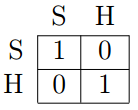
\includegraphics[width=.15\linewidth]{./images/task1a.PNG}%
          }
    \end{minipage}
    \vspace{1em}
		\textbf{Solution:}\\
		
		
		
		% Task 1b	
		\item \begin{minipage}[t]{\linewidth}
          \centering
          \adjustbox{valign=t}{%
            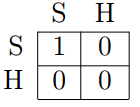
\includegraphics[width=.15\linewidth]{./images/task1b.PNG}%
          }
    \end{minipage}
    \vspace{1em}
		\textbf{Solution:}\\
		
		
		
		
		% Task 1c
		\item \begin{minipage}[t]{\linewidth}
          \centering
          \adjustbox{valign=t}{%
            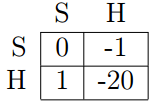
\includegraphics[width=.15\linewidth]{./images/task1c.PNG}%
          }
    \end{minipage}
    \vspace{1em}		
        \textbf{Solution:}\\
		
		
		
		% Task 1d	
		\item Interpret the results of the previous exercises. What can you say about Nash equilibria, ESS's and their relation?\\
		\textbf{Solution:}\\	
		
		
		
		
		
		
	\end{enumerate}
	
	% Task 2
	\item(Replicator Dynamics.) Consider the pairwise contest with actions A and B and payoff matrix.
	
		\begin{figure}[H]
	    \centering
  	    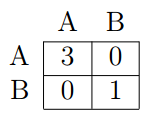
\includegraphics[width=0.15\textwidth]{images/task2.PNG}
	    \end{figure}	
	
	
	\begin{enumerate}
		% Task 2a
		\item What are the Esss of this game?\\
		\textbf{Solution:}\\
		
		
		
		
		
		
		% Task 2b
		\item Denote by $x$ the fraction of the population using A.
			\begin{enumerate}
				% Task 2b i.
				\item Compute the expected payoff of (a player with) strategy A, of strategy B, and the total expected payoff of a player.\\
				\textbf{Solution:}\\
				
				
				
				
				% Task 2b ii.
				\item Give the replicator dynamics equation for this game.\\
				\textbf{Solution:}\\
				
				
				
				
				
				% Task 2b iii.
				\item Find the fixed points.\\
				\textbf{Solution:}\\
				
				
				
				
				
				% Task 2b iv.
				\item Which fixed points are evolutionary end points? (Motivate your answer)\\
				\textbf{Solution:}\\
				
				
			\end{enumerate}
	\end{enumerate}	
	
	
	% Task 3
	\item (Experimenting with existing software.) Consider the NetLogo model available at\\ \url{http://ccl.northwestern.edu/netlogo/models/community/GameTheory}	
	
	\begin{enumerate}
		% Task 3a
		\item Run the model following the steps described in the \texttt{\#\# HOW TO USE IT} section. Try to justify the results obtained using the different setting described in the section.\\
		\textbf{Solution:}\\
		
		
		
		
		
		
		% Task 3b
		\item Discuss briefly your experience with the use of such software (pro's and con's).\\
		\textbf{Solution:}\\
		
		
		
		
	\end{enumerate}		
	
	% Task 4
	\item Consider the following sequence of states from a 1-D CA:\\
	Use the format in the scheme below (that is, specify the row 'New') to describe two sets of rules able to generate this sequence of states.
	
		\begin{figure}[H]
	    \centering
  	    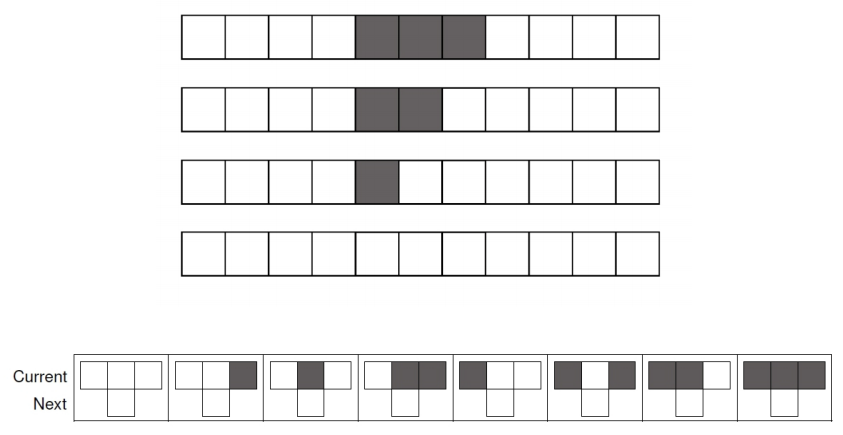
\includegraphics[width=0.7\textwidth]{images/task4.PNG}
	    \end{figure}	
	
	
	
	\textbf{Solution:}\\
	
	
	
	
	
	% Task 5
	\item Download and run the Game of Life simulator from \url{https://bitstorm.org/gameoflife/} Select "Small Exploder" from the menu, click start and wait until a stable state is eached. Explain why this state remains static.\\
	\textbf{Solution:}\\\\
	The static state looks like this:
	\begin{figure}[H]
	\centering
  	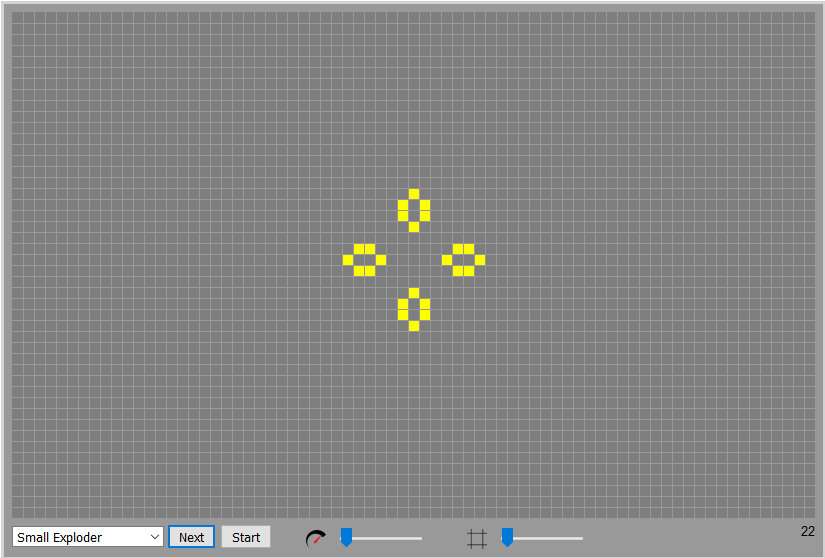
\includegraphics[width=0.7\textwidth]{images/ex_5_small_exploder.png}
	\end{figure}
	
	These structures are identical except for their orientation, we will reason about one of them, which translates to all others. The game of life has the following rules:
	\begin{itemize}
	    \item If a node is alive, and has two or three alive neighbours it stays alive
	    \item If a node is dead, it becomes alive if it has exactly three living neighbours.
	\end{itemize}
	
	We see the following properties in one of the observed static structures:
	\begin{itemize}
	    \item The two dead cells inside have five neighbours each, thus remain dead.
	    \item The alive cells each have two neighbours, thus remain alive.
	    \item The cells around the structure have a maximum of two connected living cells, thus remain dead.
	\end{itemize}
	These properties combined result in the structure remaining in a stable/static state.
	
\end{enumerate}
\end{document}